%!TEX root =SpGEMM_Accumulo_HPEC.tex

\section{Discussion}
\label{sDiscussion}

\subsection{TableMult Design Alternatives}
Our initial design operated the iterator stack on a full major compaction.
We chose to operate the iterator stack on a scan instead because major compactions experience
a delay on the order of seconds before Accumulo schedules them, slightly bumping latency,
and because opening a BatchWriter inside an iterator at major compaction presents a small chance for deadlock.
Deadlock may occur if the major compaction iterators triggered enough minor compactions 
such that they exhaust every thread in the compaction thread pool.
This leaves open the chance that a major compaction thread would block on a minor compaction thread
in order for the BatchWriter to write entries, while in turn the minor compaction thread blocks on 
the major compaction since major compactions take a higher thread pool priority than minor ones.

%bridge inner and outer product
We also believe there is room to reconsider the inner product SpGEMM formulation from our initial design
because they bottleneck on different operations: 
inner product bottlenecks heavily on scanning whereas outer product bottlenecks on writing.
See Figure~\ref{fInnerOuterSpectrum} for a pictorial comparison.
At the expense of multiple passes over input matrices, inner product emits entries more efficiently
in that emitted entries are in order and partial products can be summed immediately, 
reducing the number of entries needed to write to Accumulo to the minimum possible.
Outer product reads input matrices in a single pass
but emits %entries less efficiently in that entries emit 
entries out of order and 
has much less change to pre-sum partial products, 
requiring writing individual partial products to the result table.
For our experiment on power law input graphs, Table~\ref{tResultsParams} shows that outer product 
writes 2.5 to 3 times more entries than the minimum possible.

\begin{figure}[tbh]
\centering
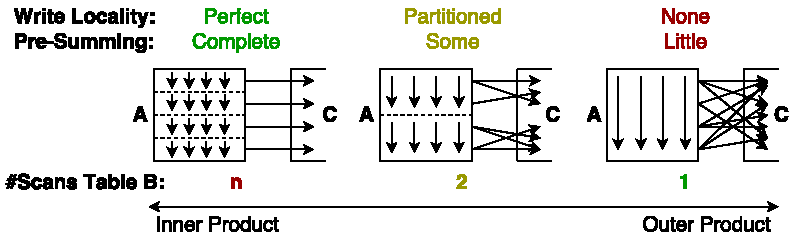
\includegraphics[width=\linewidth]{InnerOuterSpectrum}
\caption{Tradeoffs between Inner and Outer Product}
\label{fInnerOuterSpectrum}
\end{figure}

%LRU cache enables the bridge
Is it possible to blend inner and outer product algorithms and achieve better performance than either method alone?
A definitive answer is future research, though we sketch one possible bridge in Figure~\ref{fInnerOuterSpectrum}.
Suppose we partition the rows of $\matr{A}$ (columns of $\matr{A^\tr}$) into two halves 
and run outer product on each separately.
Each outer product requires scanning all of $\matr{B}$ once, for a total of two passes.
In exchange we increase write locality:
the top half outer product only writes to the top half of $\matr{C}$ and 
the bottom half outer product only writes to the bottom half of $\matr{C}$.
%We could do the same process on table $\matr{B}$ by symmetry.
Selecting the number of partitions along rows of $\matr{A}$ determines
balance between inner product (partitions between every row) and outer product (zero partitions).

A challenge for any hybrid algorithm is mapping it to Accumulo infrastructure.
We chose outer product because it most naturally fits into Accumulo, 
using for example iterators for one-pass streaming computation, 
BatchWriters to handle unsorted entry emission and Combiners to defer summation.
%Hybrid solutions might consider locality groups or transpose tables to enable column-oriented scanning
%and the distribution of tablets to tablet server cost modeling to 
We may realize greater performance by considering data distribution among tablet servers, for example, 
but such a consideration would require accessing and perhaps manipulating
Accumulo's internal state and non-public API.
We suggest this paper's approach as a balance between top performance and implementation stability.

%table cloning

%\todo[inline]{temporary tables}
\subsection{TableMult in Algorithms}
A frequent computaional pattern is to create intermediary tables in the middle of an algorithm 
that are not needed once the algorithm completes.  For example, we may have a series of TableMult operations 
for which only the final TableMult is needed as output.  It is therefore wasteful to write the intermediary
TableMult results to disk if we have room to store them in memory.
Sometimes one can restructure an algorithm to minimize the use of intermediary tables,
but a better solution would be to realize a notion of in-memory ``temporary tables'' in Accumulo.
We leave constructing this notion to future work.

Similarly, it is also useful to \emph{pipeline} TableMults in an algorithm by starting the process 
that acts on the result of a TableMult before the TableMult finishes.
Unfortunately, the outer product algorithm cannot guarantee that all partial products for a particular element 
are written to the result table before the algorithm finishes, since it writes results in chaotic order.
The inner product algorithm would be easier to pipeline.
We therefore treat TableMult operations as barriers for operations acting on a TableMult's result.

%% \todo[inline]{Probably remove next paragraph:}
%% We implemented TableMult logic inside three separate iterators connected via the SortedKeyValueIterator
%% interface. One technique for increasing performance is \emph{loop fusion}, combining separate components into one
%% that performs everything in one pass.  We chose to keep our iterators separate because it opens them 
%% to reuse in other server-side operations and the iterator's processing (including necessary decoding and encoding)
%% is not our bottleneck. We will be bound by BatchWrite time no matter how well we optimize the iterator processing.


\section{Related Work} %Analogy to MapReduce with Accumulo Scanners, Iterators and BatchWriters:
%\todo[inline]{Cannon's algorithm, other SpGEMM}
Bulu\c{c} and Gilbert have studied SpGEMM rigorously, comparing parallel message passing 
algorithm implementations, proving theoretical bounds and plotting performance \cite{buluc2012parallel}.
Most of the algorithms they present including Sparse SUMMA algorithms use 2D block decompositions.
Unfortunately, 2D decompositions are quite difficult in Accumulo 
and message passing between servers even more so.
In this work we use a 1D decomposition along rows with no tablet server communication 
other than shuffling partial products to result tablets via a BatchWriter.

Our outer product method could have been implemented in MapReduce %x\cite{dean2008mapreduce} 
on Hadoop or its successor YARN \cite{vavilapalli2013apache}.
In fact, there is a natural analogy from
how we process data using Accumulo infrastructure to methods in MapReduce.

In the map phase, we map matching rows of the input tables to a list
of partial products generated from their outer product.
We realize the map phase in Accumulo via the Scanners and the TwoTableIterator.
In the shuffle phase, we send partial products to the correct tablet of the result
table via machinery in the Accumulo BatchWriter (using data in the metadata table).
In the reduce phase, partial products are lazily combined by Accumulo combiners 
that implement the $\oplus$ operation.

We have a hunch that a MapReduce implementation using the AccumuloInputFormat and AccumuloOutputFormat 
will outperform our implementation in terms of throughput for large input tables (i.e. whole-table analytics)
but not latency for moderate input tables (i.e. queued analytics), due to spinup delay MapReduce jobs experience.
In either case, using MapReduce requires features in Hadoop clusters outside the 
Accumulo ecosystem, which may not be an option for some user environments.
It would be interesting to directly compare a MapReduce implementation in the future.


%\todo[inline]{Stored Procedures a la MySQL}

% Talk about how we measured performance?
To measure performance, we used techniques similar to those from Google Dapper \cite{sigelman2010dapper}.
We instrument sections of code inside try-finally statements, recording the start time before 
entering those sections and ensuring we record stop times inside the finally portion.
We store total time spent inside these code section ``spans'' inside thread-local storage,
along with statistics on how many times we enter a span and the minimum and maximum amount of time
spent inside a span. These statistics showed us what code was being traversed more often than expected
and what portions of code took the longest. 

\section{Conclusions}
\label{sConclusions}

In this work we showcase the design of TableMult, a Graphulo implementation of the 
SpGEMM GraphBLAS linear algebra kernal server-side on Accumulo tables.
We compare inner and outer approaches for SpGEMM and show how outer product is better
suited to the Accumulo iterator environment.
Performance experiments show ideal weak scaling and hint at good strong scaling,
although repeating our experiments on a larger cluster is necessary to confirm.

Current research is to implement the remaining GraphBLAS kernels 
and develop algorithms calling them, % atop the Graphulo library,
ultimately delivering a Graphulo linear algebra library 
as a pattern for server-side computation
to the Accumulo community.
